%
% Introdução
%
\section*{Introdução} \label{Introducao}

Com a evolução da \textit{Internet of Things (IoT)} nos dias de hoje, seria expectável que tarefas básicas do dia-a-dia se encontrassem ao abrigo destas tecnologias. Tal avanço minimizaria o tempo desperdiçado pelas pessoas. Ao automatizarmos a recolha de dados relacionada com os stocks de produtos em casa, simplificamos a gestão dos mesmos. Desta forma, auxiliamos os utilizadores a manter o stock adequado às suas necessidades, bem como alerta-lo para a falta de produtos. Assim, o nosso trabalho vai no sentido de responder a questões como: ``De que forma podemos evitar transtornos causados na altura de reabastecer a nossa despensa? Ou como proceder ao controlo de stocks de alimentos e outros produtos? Como impedir artigos fora de prazo?". Se entendermos que a nossa casa funciona como uma empresa, onde existem pessoas que podem realizar as mesmas tarefas, e.g. ir às compras seguindo uma lista previamente elaborada, capacitamos qualquer elemento da família para exercer a compra.

Para responder às perguntas levantadas anteriormente, pretendemos desenhar duas aplica-ções, uma móvel e uma web, que interagem diretamente com uma Web API. A recolha de dados, i.e., informação dos produtos existentes, é feita por um leitor de {\itshape tags} (NFC ou RFID) e transmitida para a Web API, para ser armazenada. Os locais de armazenamento de produtos devem dispor de dispositivos de hardware, equipados com scanners capazes de ler as {\itshape tags} e sensores de movimento. A adoção destas peças é a chave na monitorização dos stocks, permitindo a distinção do tipo de movimento, de entrada ou saída.

No âmbito do nosso projeto assumimos a existência de duas formas de apresentação para os produtos, avulsos e embalados. Os primeiros são conservados em sistemas de arrumação (caixas, sacos, etc.), que contém {\itshape tags} NFC programáveis por {\itshape smartphones}. Os detalhes dos produtos são especificados pelo utilizador e carregados para a {\itshape tag}. Enquanto que para os produtos embalados, admitimos que os produtores utilizam {\itshape tags}, NFC ou RFID, para guardar os rótulos em formato standard.


\vspace{-15mm}
\hspace{2mm}

\begin{figure}[h!]
	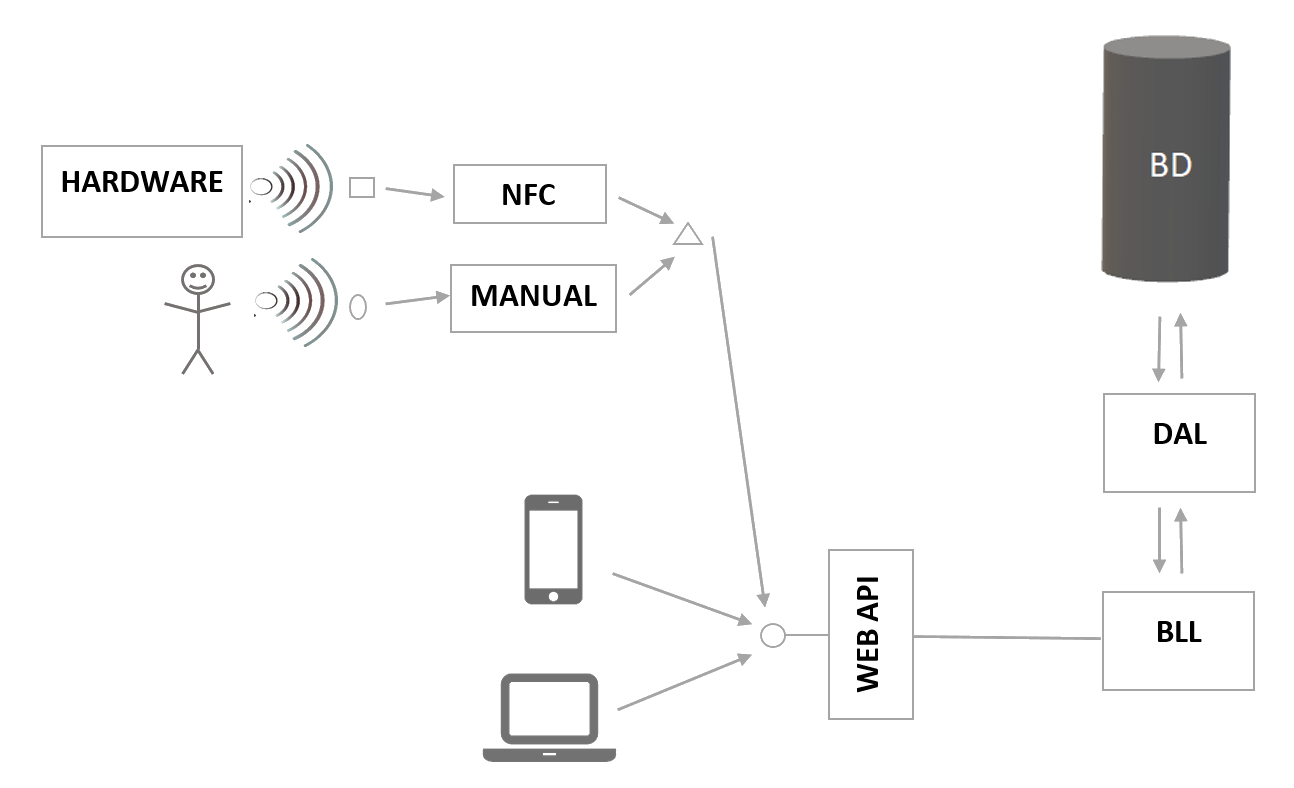
\includegraphics[width=14cm,height=7.5cm,scale=0.5]{./figures/Esquema_Estrutura_Projeto_Geral.png}
	\caption{Esquema Geral do Projeto}
	\label{esquema_geral}
\end{figure}

